%%%%%%%%%%%%%%%%%%%%%%%%%%%%%%%%%%%%%%%%%%%%%%%%%%%%%%%%%%%%%%%%%%%%%%%%%%%%%%%
% Chapter 'Adsorption - Propane - zeolite crystal 5A'
%%%%%%%%%%%%%%%%%%%%%%%%%%%%%%%%%%%%%%%%%%%%%%%%%%%%%%%%%%%%%%%%%%%%%%%%%%%%%%%
\subsection{Zeolite crystal 5A}
%
%%%%%%%%%%%%%%%%%%%%%%%%%%%%%%%%%%%%%%%%%%%%%%%%%%%%%%%%%%%%%%%%%%%%%%%%%%%%%%%
%%%%%%%%%%%%%%%%%%%%%%%%%%%%%%%%%%%%%%%%%%%%%%%%%%%%%%%%%%%%%%%%%%%%%%%%%%%%%%%
\subsubsection{DubininAstakhov - ID 1}
%
\begin{tabular}[l]{|lp{11.5cm}|}
\hline
\addlinespace

\textbf{Sorbent:} & zeolite crystal \\
\textbf{Subtype:} & 5A \\
\textbf{Refrigerant:} & Propane \\
\textbf{Equation:} & DubininAstakhov \\
\textbf{ID:} & 1 \\
\textbf{Reference:} & Grande, Carlos A.; Gigola, Carlos; Rodrigues, Alírio E. (2002): Adsorption of Propane and Propylene in Pellets and Crystals of 5A Zeolite. In: Ind. Eng. Chem. Res. 41 (1), S. 85–92. DOI: 10.1021/ie010494o. \\
\textbf{Comment:} & None \\

\addlinespace
\hline
\end{tabular}
\newline

\textbf{Properties of sorbent:}
\newline
%
\begin{longtable}[l]{lll}
\toprule
\addlinespace
\textbf{Property} & \textbf{Unit} & \textbf{Value} \\
\addlinespace
\midrule
\endhead
\bottomrule
\endfoot
\bottomrule
\endlastfoot
\addlinespace

Diameter of crystal & \si{\milli\meter} & 0.001\\

\addlinespace\end{longtable}

\textbf{Equation and parameters:}
\newline
%
Loading $w$ in $\si{\kilogram\per\kilogram}$ is calculated depending on pressure $p$ in $\si{\pascal}$, temperature $T$ in $\si{\kelvin}$, and vapor pressure $p_\mathrm{sat}$ in $\si{\pascal}$ by:
%
\begin{equation*}
\begin{split}
w &=& \begin{cases} W \rho_\mathrm{sat}^{\mathrm{liq}} & \quad \text{if flag} \geq 0 \\ W & \quad \text{else} \end{cases} & \quad\text{, and} \\
W &=& W_0 \exp \left( - \left( \nicefrac{A}{E} \right) ^{n} \right) & \quad\text{, and} \\
A &=& R T \ln \left( \nicefrac{p_\mathrm{sat}}{p} \right) & \quad\text{.} \\
\end{split}
\end{equation*}
%
The parameters of the equation are:
%
\begin{longtable}[l]{lll|lll}
\toprule
\addlinespace
\textbf{Par.} & \textbf{Unit} & \textbf{Value} &	\textbf{Par.} & \textbf{Unit} & \textbf{Value} \\
\addlinespace
\midrule
\endhead

\bottomrule
\endfoot
\bottomrule
\endlastfoot
\addlinespace

flag & - & -1.000000000e+00 & $n$ & - & 2.240000000e+00 \\
$E$ & $\si{\joule\per\mole}$ & 1.940000000e+04 & $W_0$ & $\si{\kilogram\per\kilogram}$ & 1.486170000e-01 \\

\addlinespace\end{longtable}

\textbf{Validity:}
\newline
Equation is approximately valid for $2450.0 \si{\pascal} \leq p \leq 99391.0 \si{\pascal}$,  $323.0 \si{\kelvin} \leq T \leq 423.0 \si{\kelvin}$, and $0.011807775 \si{\kilogram\per\kilogram} \leq w \leq 0.137102049 \si{\kilogram\per\kilogram}$.
\newline

\textbf{Visualization:}
%
\begin{figure}[!htp]
{\noindent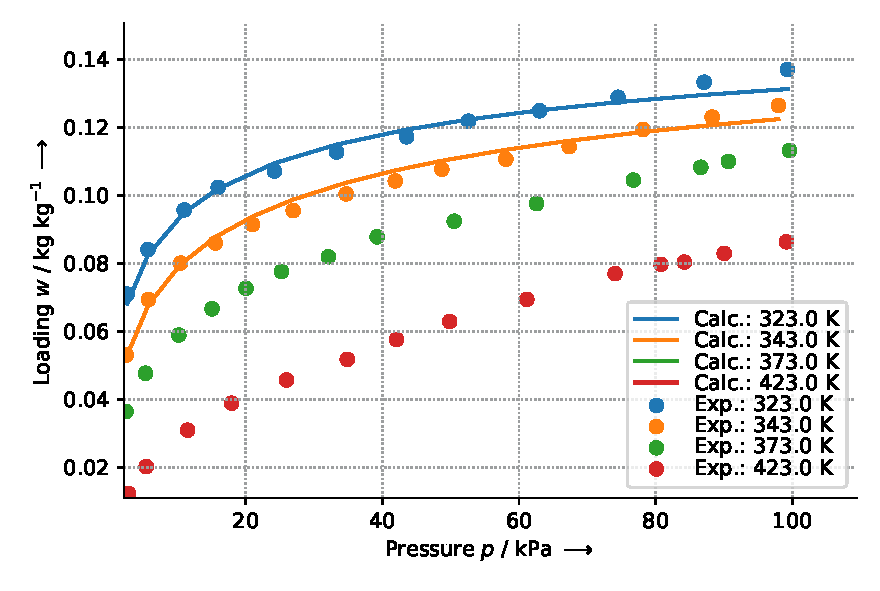
\includegraphics[height=10cm, keepaspectratio]{figs/ads/ads_Propane_zeolite_crystal_5A_DubininAstakhov_1.pdf}}
\end{figure}
%

To generate the figure, the following refrigerant functions were selected:
\begin{itemize}
\item Vapor pressure: VaporPressure\_EoS1 - ID 1
\item Saturated liquid density: SaturatedLiquidDensity\_EoS1 - ID 1
\end{itemize}

The uncertainity of the experimental data is:
\begin{itemize}
\item Data source $\,\to\,$ Data was taken from figure
\item Pressure, absolute, in $\si{\pascal}$ $\,\to\,$ 40
\end{itemize}

The mean absolute percentage error (MAPE) between the experimental and calculated data results in 2.0\%.
\FloatBarrier
\newpage
%%%%%%%%%%%%%%%%%%%%%%%%%%%%%%%%%%%%%%%%%%%%%%%%%%%%%%%%%%%%%%%%%%%%%%%%%%%%%%%
%%%%%%%%%%%%%%%%%%%%%%%%%%%%%%%%%%%%%%%%%%%%%%%%%%%%%%%%%%%%%%%%%%%%%%%%%%%%%%%
\subsubsection{Toth - ID 1}
%
\begin{tabular}[l]{|lp{11.5cm}|}
\hline
\addlinespace

\textbf{Sorbent:} & zeolite crystal \\
\textbf{Subtype:} & 5A \\
\textbf{Refrigerant:} & Propane \\
\textbf{Equation:} & Toth \\
\textbf{ID:} & 1 \\
\textbf{Reference:} & Grande, Carlos A.; Gigola, Carlos; Rodrigues, Alírio E. (2002): Adsorption of Propane and Propylene in Pellets and Crystals of 5A Zeolite. In: Ind. Eng. Chem. Res. 41 (1), S. 85–92. DOI: 10.1021/ie010494o. \\
\textbf{Comment:} & None \\

\addlinespace
\hline
\end{tabular}
\newline

\textbf{Properties of sorbent:}
\newline
%
\begin{longtable}[l]{lll}
\toprule
\addlinespace
\textbf{Property} & \textbf{Unit} & \textbf{Value} \\
\addlinespace
\midrule
\endhead
\bottomrule
\endfoot
\bottomrule
\endlastfoot
\addlinespace

Diameter of crystal & \si{\milli\meter} & 0.001\\
Diameter of pore & \si{\milli\meter} & 0.00005\\
Diameter of pellet & \si{\milli\meter} & 1.65-2.5\\
Porosity of pellet & - & 0.35\\
Pellet density & \si{\kilogram\per\cubic\meter} & 1130\\
Solid density & \si{\kilogram\per\cubic\meter} & 1740\\

\addlinespace\end{longtable}

\textbf{Equation and parameters:}
\newline
%
Loading $w$ in $\si{\kilogram\per\kilogram}$ is calculated depending on pressure $p$ in $\si{\pascal}$ and temperature $T$ in $\si{\kelvin}$ by:
%
\begin{equation*}
\begin{split}
w &=& \frac{w_\mathrm{sat} b^{m} p}{\left( 1 + b^{r} p^{n} \right)^{\nicefrac{1}{n}}} & \quad\text{, and} \\
b &=& b_0 \exp\left( \frac{Q^{*}}{T} \right) & \quad\text{, and} \\
n &=& n_0 + \nicefrac{c}{T} & \quad\text{, and} \\
r &=& \begin{cases} n & \quad \text{if } r^{*} < 0 \\ r^{*}  & \quad \text{else} \end{cases} & \quad\text{.}
\end{split}
\end{equation*}
%
The parameters of the equation are:
%
\begin{longtable}[l]{lll|lll}
\toprule
\addlinespace
\textbf{Par.} & \textbf{Unit} & \textbf{Value} &	\textbf{Par.} & \textbf{Unit} & \textbf{Value} \\
\addlinespace
\midrule
\endhead

\bottomrule
\endfoot
\bottomrule
\endlastfoot
\addlinespace

$b_0$ & $\si{\per\pascal}$ & 1.792538349e-04 & $Q^{*}$ & $\si{\kelvin}$ & 1.828139797e+03 \\
$c$ & $\si{\kelvin}$ & 0.000000000e+00 & $r^{*}$ & - & 1.000000000e+00 \\
$m$ & - & 2.173913043e+00 & $w_\mathrm{sat}$ & $\si{\kilogram\per\kilogram}$ & 1.605130800e-01 \\
$n_0$ & - & 4.600000000e-01 & & & \\

\addlinespace\end{longtable}

\textbf{Validity:}
\newline
Equation is approximately valid for $2475.3 \si{\pascal} \leq p \leq 99591.1 \si{\pascal}$,  $323.0 \si{\kelvin} \leq T \leq 423.0 \si{\kelvin}$, and $0.012344073 \si{\kilogram\per\kilogram} \leq w \leq 0.137030546 \si{\kilogram\per\kilogram}$.
\newline

\textbf{Visualization:}
%
\begin{figure}[!htp]
{\noindent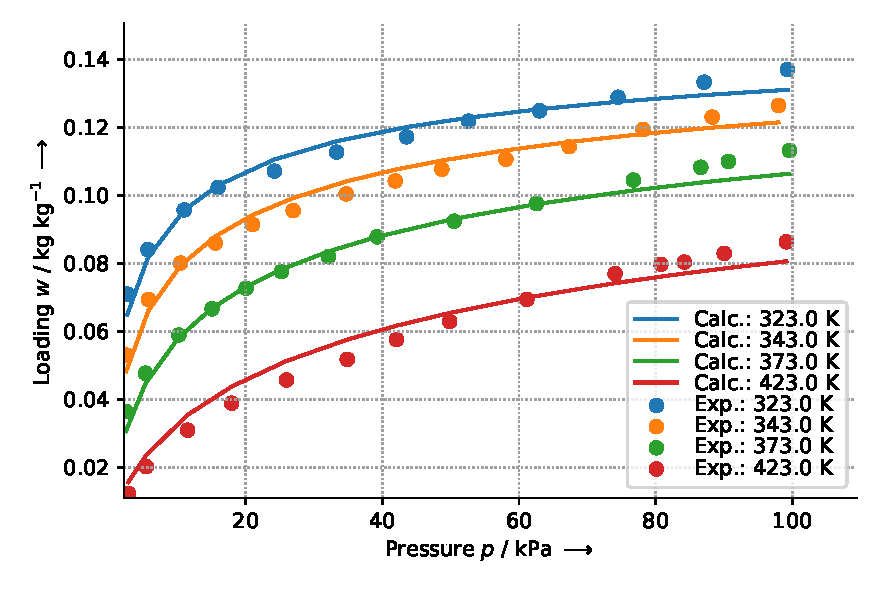
\includegraphics[height=10cm, keepaspectratio]{figs/ads/ads_Propane_zeolite_crystal_5A_Toth_1.pdf}}
\end{figure}
%

To generate the figure, the following refrigerant functions were selected:
\begin{itemize}
\item Vapor pressure: VaporPressure\_EoS1 - ID 1
\item Saturated liquid density: SaturatedLiquidDensity\_EoS1 - ID 1
\end{itemize}

The uncertainity of the experimental data is:
\begin{itemize}
\item Data source $\,\to\,$ Data was taken from figure
\item Pressure, absolute, in $\si{\pascal}$ $\,\to\,$ 40
\end{itemize}

The mean absolute percentage error (MAPE) between the experimental and calculated data results in 4.61\%.
\FloatBarrier
\newpage
%%%%%%%%%%%%%%%%%%%%%%%%%%%%%%%%%%%%%%%%%%%%%%%%%%%%%%%%%%%%%%%%%%%%%%%%%%%%%%%
